
\vspace{0.3cm}
\begin{enumerate}
    \item (25\%) Un juego utiliza una baraja de $n$ cartas diferentes, donde $n$ es un número entero y $n \geq 6.$ El número de conjuntos posibles de 6 cartas que se pueden extraer de la baraja es 6 veces el número de conjuntos posibles de 3 cartas que se pueden extraer. Encuentra $n$.\vspace{0.3cm}


    
    \item (25\%) Muchos estados utilizan una secuencia de tres letras de entre un alfabeto de 26 letras seguidas de una secuencia de tres dígitos como patrón estándar de matrícula. Dado que cada disposición de tres letras y tres dígitos es igualmente probable, la probabilidad de que dicha matrícula contenga al menos un palíndromo (una disposición de tres letras o una disposición de tres dígitos que se lea igual de izquierda a derecha que hace de derecha a izquierda) es $\dfrac{m}{n}$, donde $m$ y $n$ son números enteros positivos coprimos. Encuentre $m+n$. \textbf{Sugerencia}: La probabilidad de que un evento ocurra es $\displaystyle \frac{\text{casos favorables}}{\text{casos posibles}}$, 
\vspace{0.3cm}
 
    \item (25\%) ¿Cuántas ternas de enteros positivos $(x,y,z)$ hay de tal manera que
\[\frac{x^2+y^2}{z}< 7,\]
y cada componente está sujeta a $x\leq 8$, $y\leq 8$ y $z\leq 5$? \vspace{0.3cm}


    \item (25\%) Dada la siguiente cuadrícula, determina la cantidad de caminos $A$ a $B$ de longitud mínima.

    \begin{center}
        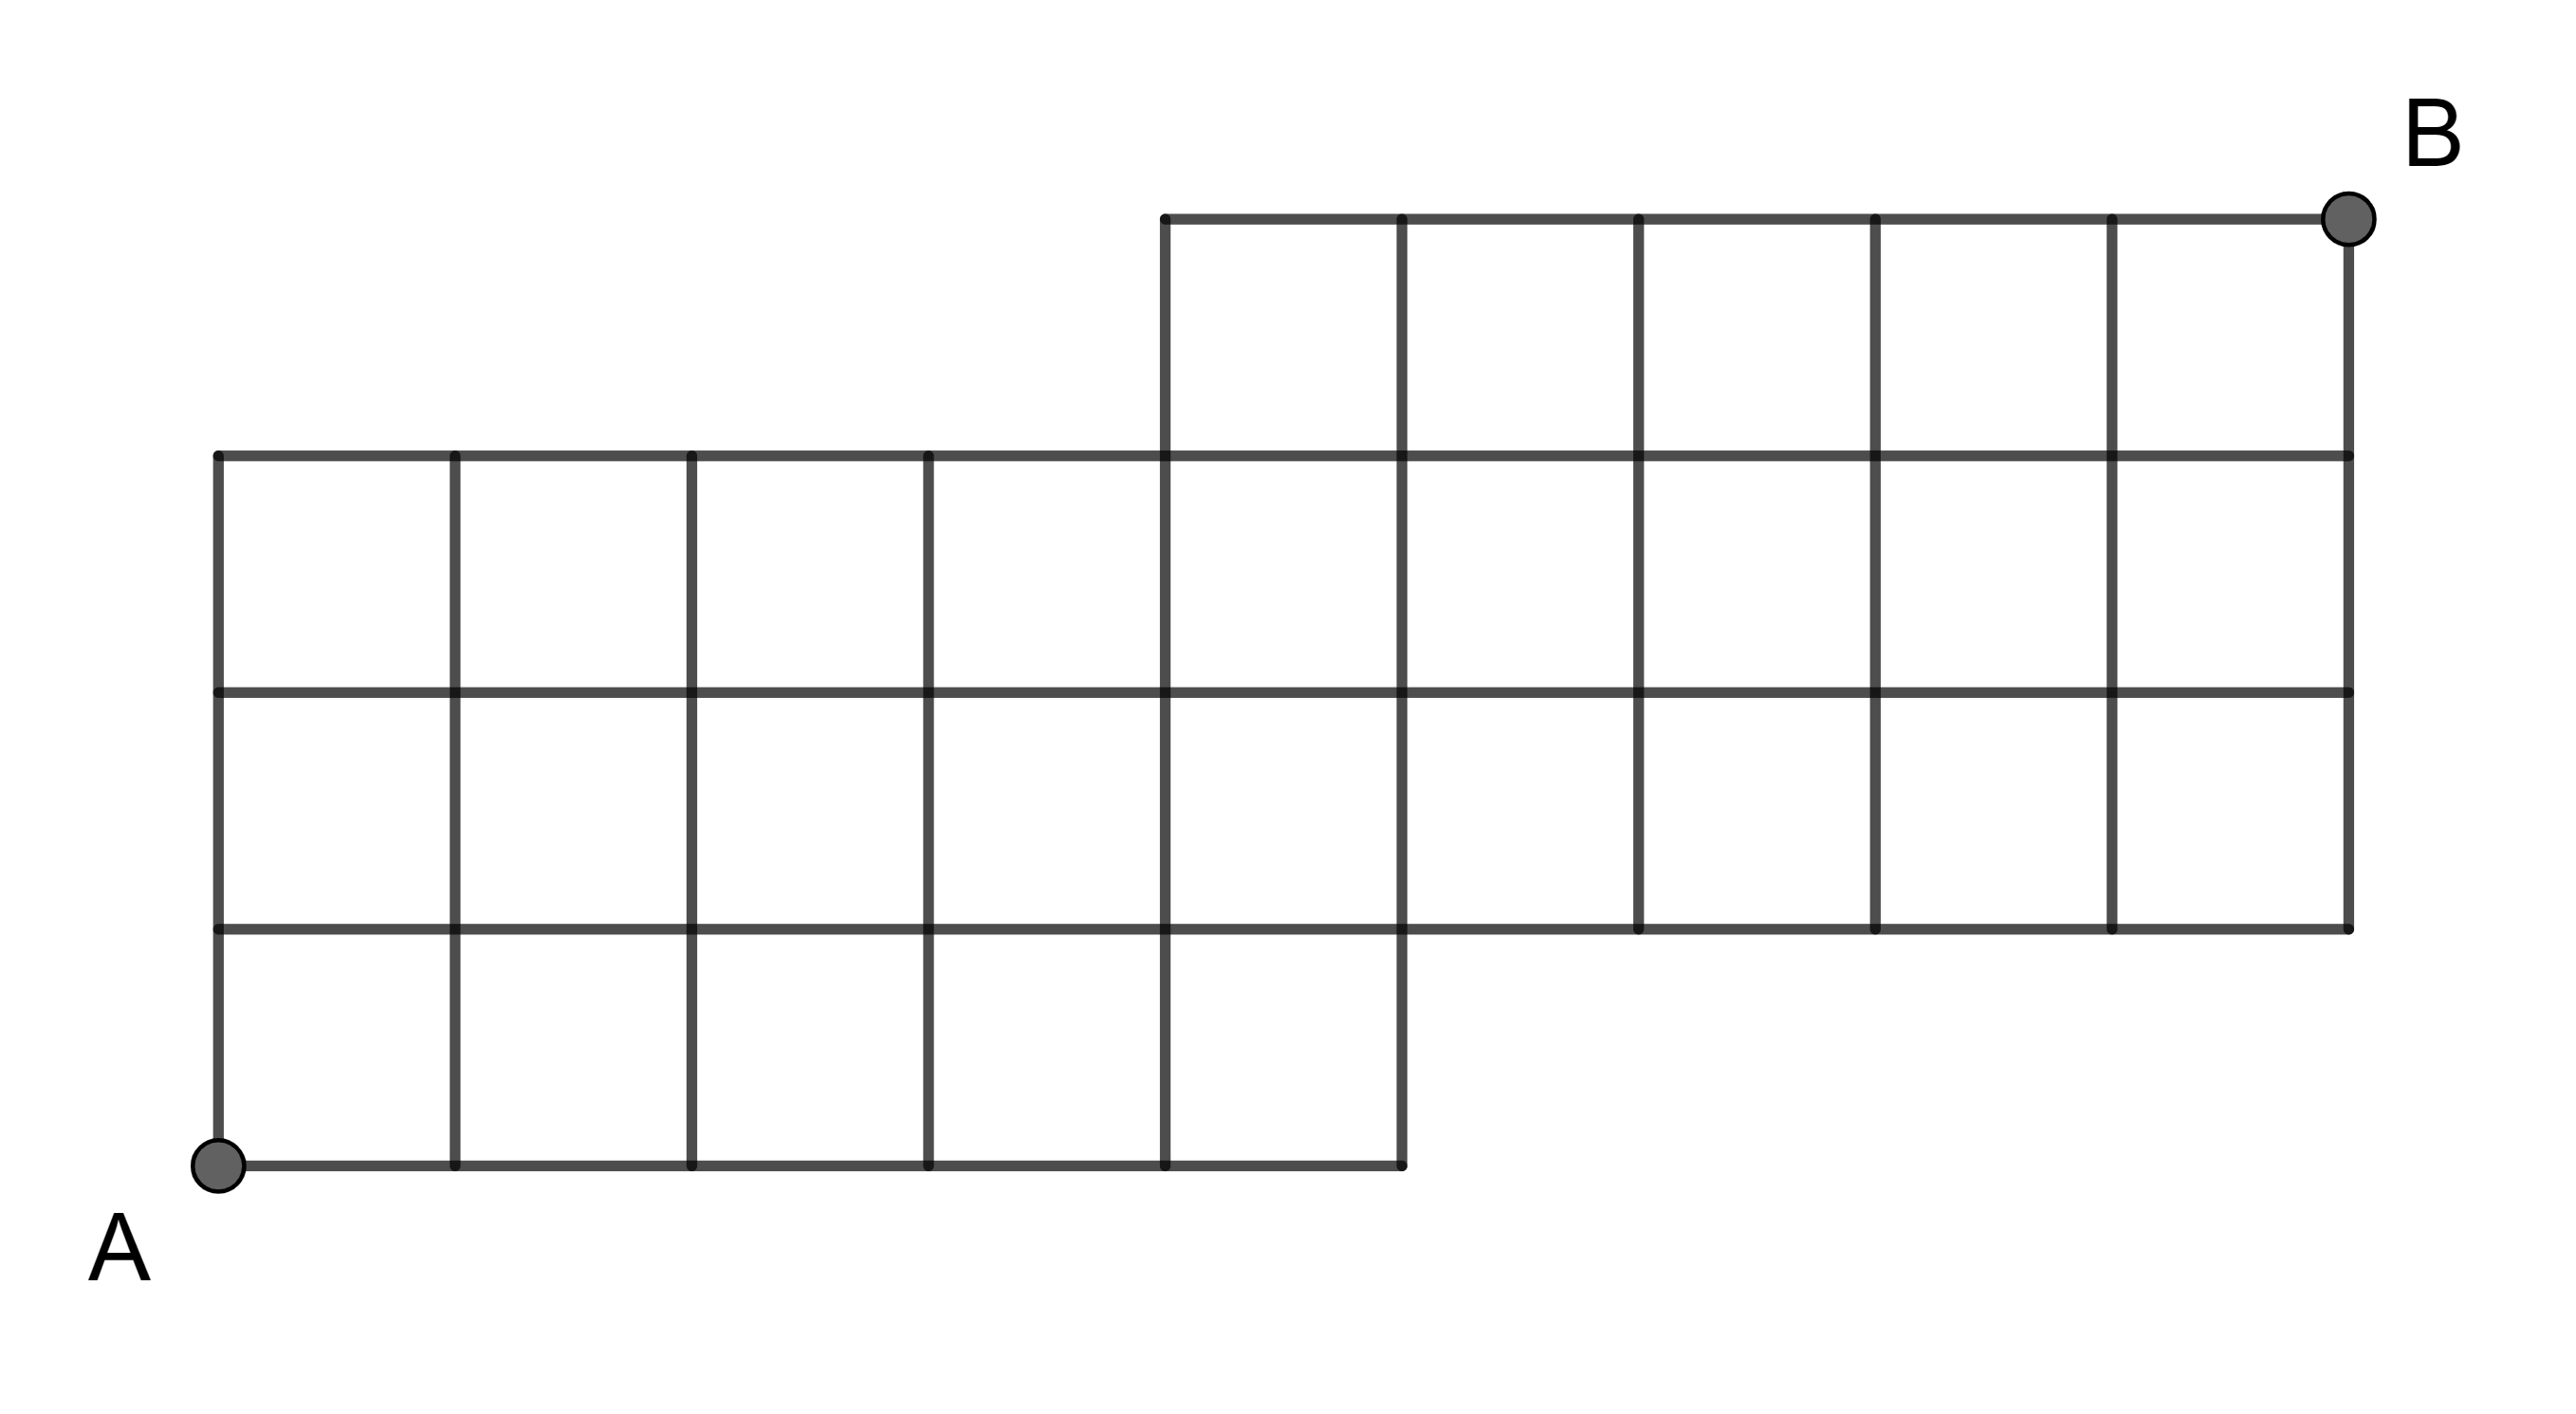
\includegraphics[scale=0.65]{Imagenes/S1/s1.png}
    \end{center}

    
\end{enumerate}

\textbf{Crédito Extra:} Se toma el elemento mayor de cada subconjunto de 7 elementos del conjunto $\{ 1,2,3,4,5,6,7,8,9,10 \}$. ¿Cuál es la suma de todos esos elementos mayores?